\documentclass[11pt]{article}
\usepackage[margin=1in]{geometry}
\usepackage{graphicx}
\usepackage{amsmath}
\usepackage{amssymb}
\usepackage{float}
\usepackage{subcaption}

\title{July 22, 2021 Meeting Agenda}

\begin{document}
\maketitle

\section{Capacity Estimation}
  \subsection{Summary Statistics}
    \begin{table}[H]
      \centering
      \caption{Summary Statistics for each work type. Share Plea is the share of days in which we observe at least one plea. ShareTrial and ShareEmpty are defined similarly. Share is the work type's share of all work types.}
      \label{tab:my-table}
      \begin{tabular}{|l|l|l|l|l|l|}
      \hline
      \textbf{WorkType} & \textbf{Days} & \textbf{Share} & \textbf{SharePlea} & \textbf{ShareTrial} & \textbf{ShareEmpty} \\ \hline
      AW          & 125.50   & 0.01 & 0.04 & 0.00 & 0.96 \\ \hline
      CP          & 3,112.67 & 0.25 & 0.03 & 0.00 & 0.97 \\ \hline
      CP CC       & 10.17    & 0.00 & 0.00 & 0.00 & 1.00 \\ \hline
      CP/PCR      & 14.50    & 0.00 & 0.03 & 0.00 & 0.97 \\ \hline
      CPNJ        & 1,300.33 & 0.11 & 0.03 & 0.00 & 0.97 \\ \hline
      CPNJ CC     & 11.00    & 0.00 & 0.36 & 0.00 & 0.64 \\ \hline
      CPNJ/GS     & 0.50     & 0.00 & 1.00 & 0.00 & 0.00 \\ \hline
      CPNJ/PCR    & 289.50   & 0.02 & 0.04 & 0.00 & 0.96 \\ \hline
      Capital PCR & 11.00    & 0.00 & 0.00 & 0.00 & 1.00 \\ \hline
      GS          & 4,160.67 & 0.34 & 0.64 & 0.05 & 0.34 \\ \hline
      GS CC       & 75.67    & 0.01 & 0.39 & 0.07 & 0.56 \\ \hline
      GS CP CC    & 53.00    & 0.00 & 0.36 & 0.06 & 0.58 \\ \hline
      GS(SGJ)     & 70.67    & 0.01 & 0.33 & 0.07 & 0.65 \\ \hline
      GS(SGJ) CC  & 0.33     & 0.00 & 0.00 & 0.00 & 1.00 \\ \hline
      GS(SGJ) CP  & 5.00     & 0.00 & 0.60 & 0.00 & 0.40 \\ \hline
      X           & 765.00   & 0.06 & 0.01 & 0.00 & 0.99 \\ \hline
      X-          & 1.00     & 0.00 & 0.00 & 0.00 & 1.00 \\ \hline
      XX          & 80.00    & 0.01 & 0.00 & 0.00 & 1.00 \\ \hline
      in chambers & 1,488.50 & 0.12 & 0.01 & 0.00 & 0.99 \\ \hline
      na          & 546.00   & 0.04 & 0.03 & 0.00 & 0.97 \\ \hline
      \end{tabular}
    \end{table}

  \subsection{Judge schedules leading up to trials}
    Suppose a judge $j$ sentenced a trial on day $d$ in county $c$. I looked at
    judge $j$'s activity in county $c$ in the three weeks leading up to $d$ and I counted the
    number of empty days we observed. I did this for all trials and plotted a histogram of the number
    of empty days. The first includes all trials, and the second is only for trials that happened on
    non-GS days. I also looked at the distribution of the work types of the empty days preceding the trials. \textbf{Takeaway:} 5 seems to be the most common number of empty days preceding a trial, for both all trials and non-GS trials. I am not sure what to make of the distribution of the work types of the days preceding the trials. For non GS trials, the most days leading up to the trial are GS, for all trials, most days leading up to the trial are CP, followed by GS.

    \begin{figure}[H]
      \centering
      \caption{Histogram of number of empty days in county preceding trial, all trials}
      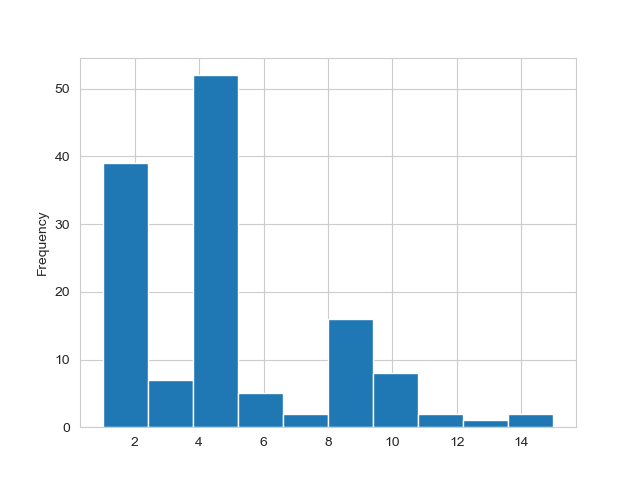
\includegraphics[width=0.65\textwidth]{../../../output/figures/Exploration/empty_days_hist_All.png}
    \end{figure}

    \begin{figure}[H]
      \centering
      \caption{Distribution of work type of empty days preceding a trial, all trials}
      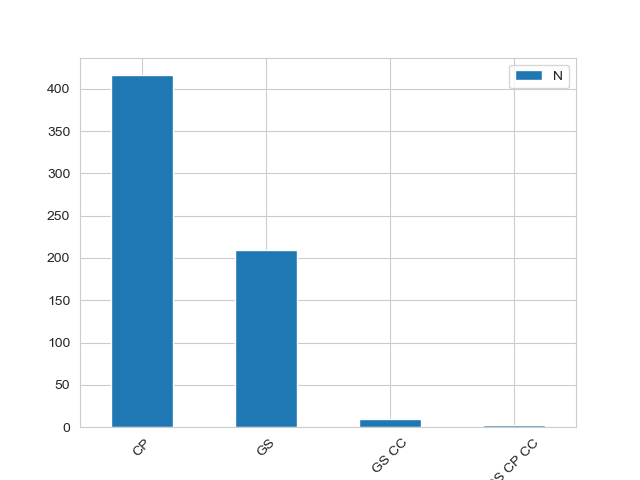
\includegraphics[width=0.65\textwidth]{../../../output/figures/Exploration/empty_days_work_type_All.png}
    \end{figure}

    \begin{figure}[H]
      \centering
      \caption{Histogram of number of empty days in county preceding trial, non-GS trials}
      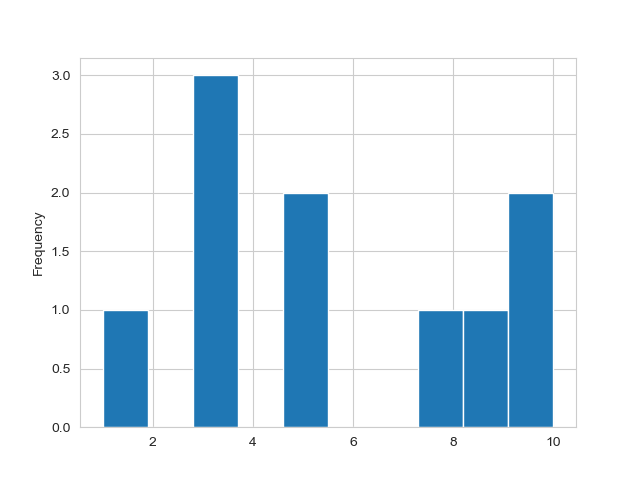
\includegraphics[width=0.65\textwidth]{../../../output/figures/Exploration/empty_days_hist_NonGS.png}
    \end{figure}

    \begin{figure}[H]
      \centering
      \caption{Distribution of work type of empty days preceding a trial, non-GS trials}
      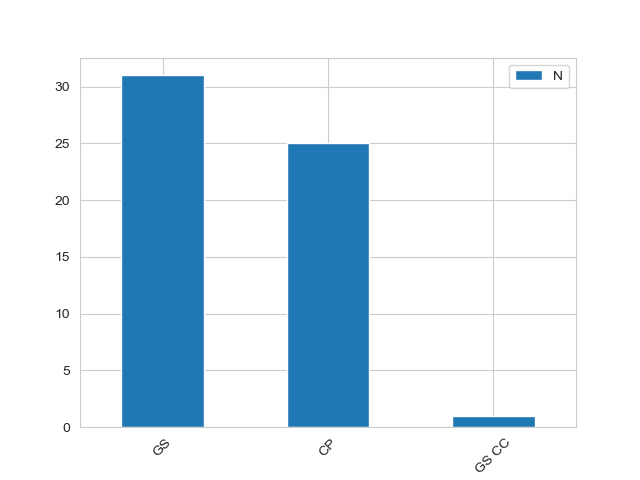
\includegraphics[width=0.65\textwidth]{../../../output/figures/Exploration/empty_days_work_type_NonGS.png}
    \end{figure}

\section{Trial Scheduling in Simulation}

  \subsection{Travel probability}
    \begin{table}[H]
      \centering
      \small
      \caption{Probability of being in county, in circuit, and out of circuit for each judge}
      \begin{tabular}{|l|l|l|l|}
      \hline
      \textbf{JudgeID} & \textbf{County} & \textbf{Circuit} & \textbf{Out of Circuit} \\ \hline
      Judge 1          & 0.38            & 0.10             & 0.52                 \\ \hline
      Judge 10         & 0.08            &                  & 0.92                 \\ \hline
      Judge 11         & 0.66            & 0.20             & 0.15                 \\ \hline
      Judge 12         & 0.25            & 0.05             & 0.70                 \\ \hline
      Judge 13         & 0.23            & 0.22             & 0.55                 \\ \hline
      Judge 14         & 0.15            & 0.05             & 0.80                 \\ \hline
      Judge 15         & 0.09            &                  & 0.91                 \\ \hline
      Judge 16         & 0.22            & 0.07             & 0.71                 \\ \hline
      Judge 17         & 0.44            & 0.34             & 0.23                 \\ \hline
      Judge 18         & 0.37            & 0.13             & 0.50                 \\ \hline
      Judge 19         & 0.16            &                  & 0.84                 \\ \hline
      Judge 2          & 0.13            &                  & 0.87                 \\ \hline
      Judge 20         & 0.24            & 0.18             & 0.58                 \\ \hline
      Judge 21         & 0.31            & 0.21             & 0.47                 \\ \hline
      Judge 22         & 0.29            & 0.15             & 0.55                 \\ \hline
      Judge 23         & 0.44            & 0.20             & 0.37                 \\ \hline
      Judge 24         & 0.42            & 0.11             & 0.47                 \\ \hline
      Judge 25         &                 &                  & 1.00                 \\ \hline
      Judge 26         & 0.32            & 0.18             & 0.50                 \\ \hline
      Judge 27         & 0.41            & 0.20             & 0.39                 \\ \hline
      Judge 28         & 0.23            & 0.14             & 0.62                 \\ \hline
      Judge 29         & 0.27            & 0.22             & 0.51                 \\ \hline
      Judge 3          & 0.20            & 0.07             & 0.73                 \\ \hline
      Judge 30         & 0.35            & 0.08             & 0.56                 \\ \hline
      Judge 31         & 0.15            &                  & 0.85                 \\ \hline
      Judge 32         & 0.11            &                  & 0.89                 \\ \hline
      Judge 33         & 0.27            & 0.12             & 0.61                 \\ \hline
      Judge 34         & 0.24            & 0.17             & 0.58                 \\ \hline
      Judge 35         & 0.41            & 0.08             & 0.51                 \\ \hline
      Judge 36         & 0.15            &                  & 0.85                 \\ \hline
      Judge 37         & 0.13            &                  & 0.87                 \\ \hline
      Judge 38         & 0.15            &                  & 0.85                 \\ \hline
      Judge 39         & 0.12            &                  & 0.88                 \\ \hline
      Judge 4          & 0.38            & 0.08             & 0.54                 \\ \hline
      Judge 40         & 0.67            & 0.15             & 0.19                 \\ \hline
      Judge 41         & 0.75            & 0.15             & 0.10                 \\ \hline
      Judge 42         & 0.24            & 0.07             & 0.69                 \\ \hline
      Judge 43         & 0.26            & 0.22             & 0.52                 \\ \hline
      Judge 44         & 0.26            & 0.15             & 0.59                 \\ \hline
      Judge 45         & 0.26            & 0.23             & 0.51                 \\ \hline
      Judge 46         & 0.02            & 0.03             & 0.95                 \\ \hline
      Judge 47         & 0.41            & 0.20             & 0.39                 \\ \hline
      Judge 48         & 0.14            &                  & 0.86                 \\ \hline
      Judge 49         & 0.31            & 0.19             & 0.50                 \\ \hline
      Judge 5          & 0.11            &                  & 0.89                 \\ \hline
      Judge 50         & 0.18            & 0.02             & 0.79                 \\ \hline
      Judge 6          & 0.11            &                  & 0.89                 \\ \hline
      Judge 7          &                 &                  & 1.00                 \\ \hline
      Judge 8          & 0.21            & 0.16             & 0.63                 \\ \hline
      Judge 9          & 0.24            & 0.08             & 0.68                 \\ \hline
      \end{tabular}
    \end{table}

  \subsection{Trials by Resident vs Non-Resident Judges by County}
    To determine each judge's home county, I used Rhys's home circuit assignments to determine each judge's home circuit. For those judges that had a home circuit, I made their home county the county to which they are assigned to the most days according to the calendar data. In the histograms below, the blue bars are the number of trials heard by a non-resident judge, and the red bars are the number of trials heard by a resident judge.  Overall, it still looks like it is common for non-resident judges to hear trials in each county.
      \begin{figure}[H]
        \centering
        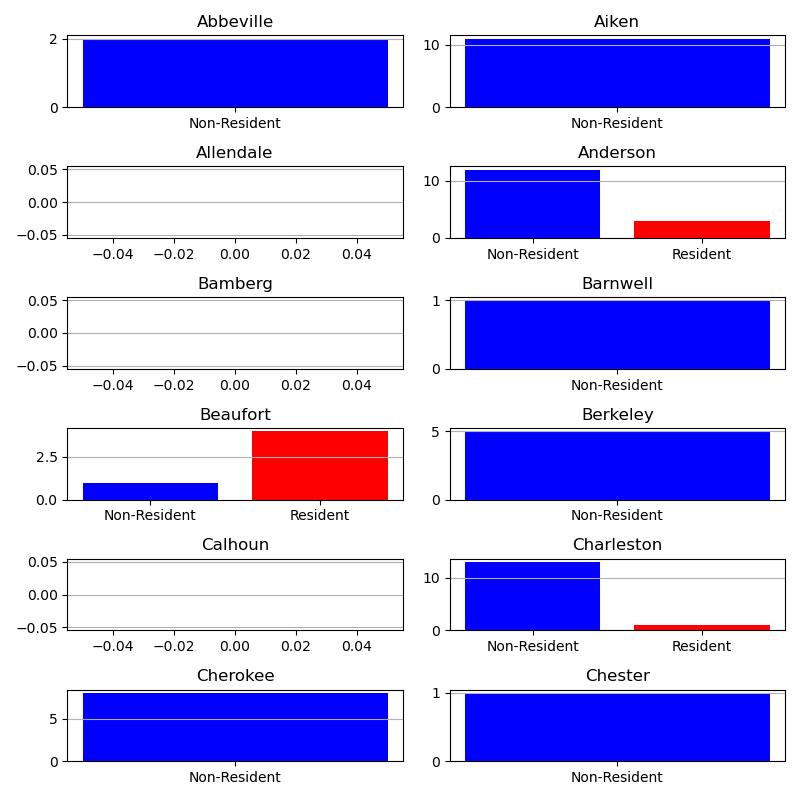
\includegraphics[width=0.9\textwidth]{../../../output/figures/Exploration/county_trial_hist_0.png}
      \end{figure}

      \begin{figure}[H]
        \centering
        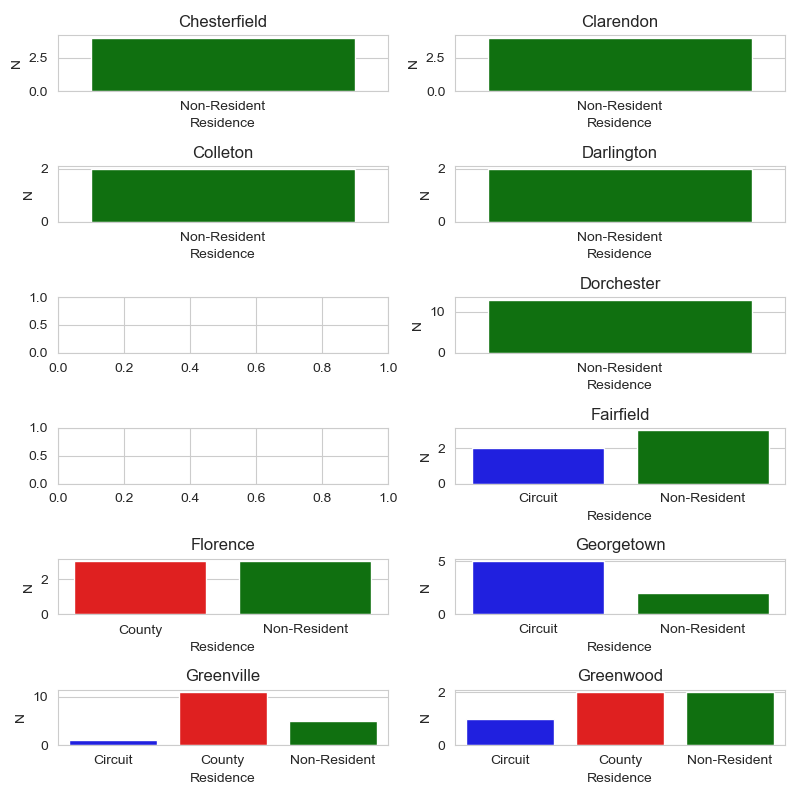
\includegraphics[width=0.9\textwidth]{../../../output/figures/Exploration/county_trial_hist_1.png}
      \end{figure}

      \begin{figure}[H]
        \centering
        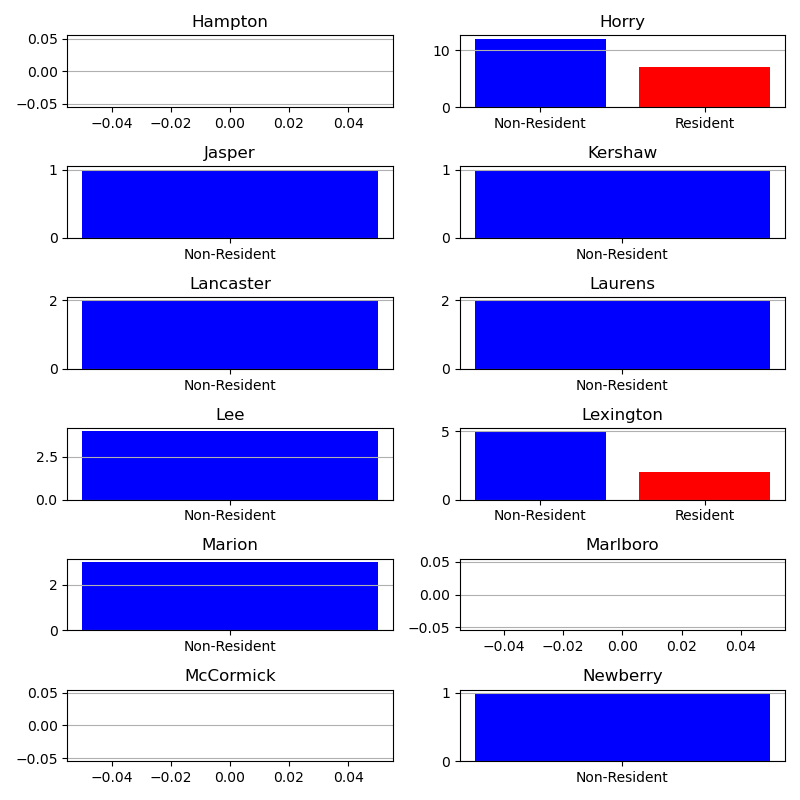
\includegraphics[width=0.9\textwidth]{../../../output/figures/Exploration/county_trial_hist_2.png}
      \end{figure}

      \begin{figure}[H]
        \centering
        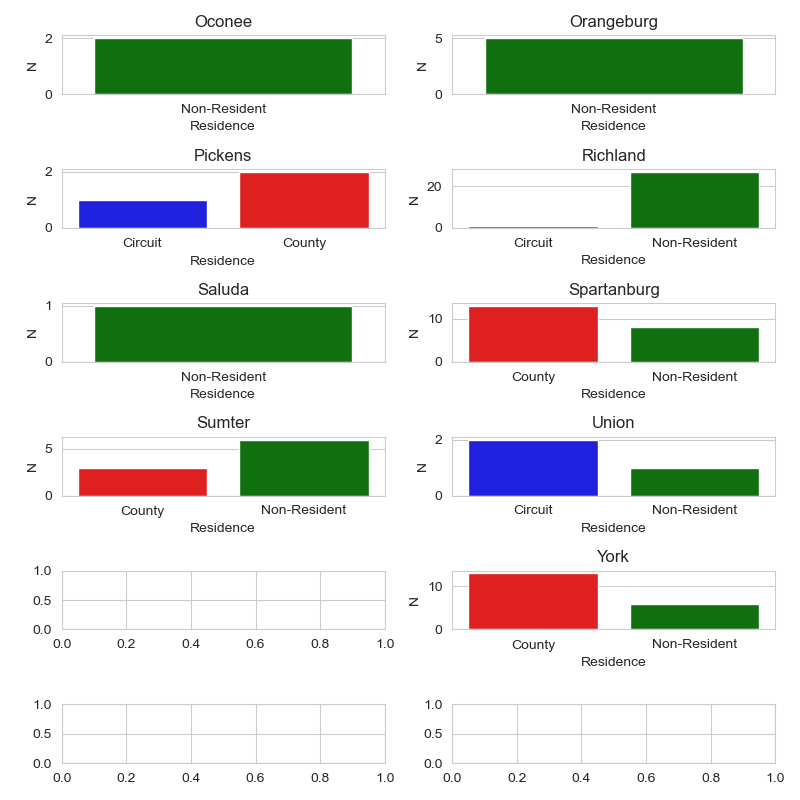
\includegraphics[width=0.9\textwidth]{../../../output/figures/Exploration/county_trial_hist_3.png}
      \end{figure}

\end{document}
